% -*- coding: utf-8; -*-

\chapter{Introduction}

So, to start with, could you provide me with more details about your research idea? What specific area in the field of programming languages are you interested in? What problem or question would you like your research to address?

Sure. I'll provide you with more details about our research idea. I will present you some background information so we can formulate an enthralling laconic research proposal for our target audience.

I am interested in Typing Mutable References. The main reference for the problem my research adresses is the Software Foundations series by Benjamin C. Pierce. The first two volumes, "Logical Foundations" and "Programming Language Foundations" gives a solid understanding of "functional programming, basic concepts of logic, computer-assisted theorem proving, and Coq." and also "the theory of programming languages, including operational semantics and static type systems." respectively. More specifically, the chapter "References" contains a very interesting implementation of mutable references in a Simply Typed Lambda Calculus (STLC) language that we take as an inspiration for condcting our study aroud typing mutable references.


Summaries:

--------------------------------------------1-------------------------------------
```
Title: Typing Mutable References in Functional Programming Languages: An Exploration Rooted in Software Foundations
Summary

This research aims to delve into the realm of mutable references in functional programming languages, specifically in Simply Typed Lambda Calculus (STLC), using the Software Foundations series by Benjamin C. Pierce as a principal reference. We are motivated by the goal of enhancing the mathematical foundation of reliable software, an objective that requires a comprehensive understanding of functional programming, logic, computer-assisted theorem proving, and the Coq proof assistant.

Software Foundations series is notable for its unique approach in presenting its material: it is entirely formalized and machine-checked, serving not just as a traditional textbook but also as a script for the Coq proof assistant. This series presents topics such as logic, proof assistants, and functional programming, tying these concepts intricately together and illustrating their interconnectedness in computer science.

Our research will further expand on these concepts by investigating mutable references, a topic inspired by a chapter within the Software Foundations series. Mutable references are a key aspect of programming languages, and understanding them in the context of functional programming could provide useful insights into software reliability.

The exploratory journey will be steered using the Coq proof assistant, a tool designed to construct proofs of logical propositions. Coq has been a significant enabler in computer science and mathematics, providing a robust platform for modeling programming languages, developing formally certified software, and functional programming. By using Coq as our primary tool, we aim to extend our understanding of mutable references, eventually contributing to the development of more reliable and efficient software systems.

In essence, this research represents an ambitious attempt to intertwine functional programming, theorem proving, and typing mutable references in the interest of advancing the underpinnings of dependable software development.
```
---------------------------------------------------------------------------------

--------------------------------------------2-------------------------------------
```
This section delves into the intricate differences and similarities between formal and informal mathematical proofs. The narrative revolves around the argument that a proof, at its core, is a means of communication.

On one hand, a formal proof is considered a set of instructions or 'code' that can guide a mechanical program, such as Coq, to derive the truth of a proposition from a set of logical rules. Its precise nature makes it suitable for a machine to follow and derive the desired conclusion. The key example used is the Coq proof of the associative property of addition.

On the other hand, an informal proof can be thought of as an 'algorithm', more suited to human understanding, using natural languages such as English. The success of an informal proof is dependent on its ability to convince its human reader of the truth of a proposition. However, as the section elucidates, the persuasiveness of an informal proof can vary from reader to reader due to differences in experience, knowledge, and personal preference.

The two types of proofs are further compared using the theorem that addition is associative. Here, a detailed side-by-side comparison is provided between a formal proof in Coq and a more traditional, informal proof that a mathematician might write. The informal proof is found to be more comprehensive in providing intermediate updates about the "proof state," although it lacks some explicit details present in the formal proof.

Despite the differences, both formal and informal proofs have their unique strengths and are essential for different purposes. Formal proofs excel in situations where absolute precision is necessary, such as computer programs. On the other hand, informal proofs are more effective in communicating complex mathematical ideas among humans due to their adaptable and intuitive nature. Therefore, one cannot be entirely preferred over the other; both coexist and serve their unique purposes in the realm of mathematical proofs.
```
---------------------------------------------------------------------------------

--------------------------------------------3-------------------------------------

```
Summary: Programming Language Foundations Preface Introduction

This book offers a comprehensive exploration of fundamental concepts in the mathematical study of programs and programming languages. Its target audience ranges from advanced undergraduate students to PhD candidates and researchers. The book employs the Coq proof assistant, a tool used to formalize mathematical proofs, throughout its discussions.

The book is structured into core chapters and additional offshoots, providing material for half a semester's course. It builds on the contents of Logical Foundations (the first volume in the Software Foundations series), and it can be used either in conjunction with that book or as a standalone resource.

The book explores two main themes: (1) the use of formal techniques to reason about the properties of specific programs, such as proving that a specific sorting function or compiler adheres to a formal specification; and (2) the use of type systems to provide assurance that all programs in a given language behave in a certain way.

In the first part, the book delves into program verification. It introduces ways to represent programs mathematically and describes their behaviors using abstract syntax and operational semantics. The first programming language discussed in detail is Imp, a simple language that embodies the essential features of conventional imperative programming. Two methods are used to reason about the properties of Imp programs: equivalence (based on their behavior in any initial memory state) and Hoare triples (programs annotated with pre- and post-conditions about memory states).

The second major topic is type systems. The book elaborates on how type systems are lightweight formal methods that can be built into compilers or program analyzers. This section also links back to the start of the book, as it explores the simply typed lambda-calculus, a model that closely represents the core of Coq.
```

---------------------------------------------------------------------------------

--------------------------------------------4-------------------------------------

```
Summary

This chapter delves into the incorporation of mutable references in programming languages, focusing on their roles as computational effects that facilitate more than mere return of results. They allow for dynamic variable alteration, execution of input and output tasks, and management of control transfers. Mutable references necessitate the explicit handling of a 'store' or 'heap', as well as 'pointers' which indicate store locations.

The approach to mutable references varies across different programming languages. For instance, ML keeps name-binding and assignment separate, with variables either holding values or pointers to mutable cells. Conversely, languages such as C or Java treat all variables as mutable cells with automatic dereferencing.

To illustrate mutable references, the chapter extends the simply-typed lambda calculus with natural numbers. Key operators introduced include 'ref' for allocating a reference, '!' for dereferencing to read the current cell value, and ':=' for assignment to alter the value stored in a cell. The understanding of these mechanisms paves the way for more advanced concepts in programming language semantics.
```

---------------------------------------------------------------------------------

--------------------------------------------5-------------------------------------

```
Summary

This section further explores mutable references in programming, particularly the implications and utility of typing, references, aliasing, shared state, objects, compound references, null references, and garbage collection.

The preliminary typing rules for allocation, dereferencing, and assignment are outlined using an informal notation. The creation of aliases, or different variables pointing to the same memory cell, is discussed in-depth due to its capability to make programs complex and yet valuable, enabling shared state or "implicit communication channels" between different program parts.

The usefulness of references becomes more prominent as they are employed in creating objects and shared state, and are even used for more advanced structures, such as mutable lists and trees. Mutable references to compound types such as functions and other references are also covered, demonstrating their application in implementing structures like arrays of numbers.

Null references, a common element in C-like languages, are discussed. The pitfalls of such pointers, including potential program failure and significant trouble they cause, are highlighted. However, the use of sum types is proposed as an efficient way to handle such situations, avoiding the need to extend basic reference mechanisms.

Finally, the topic of garbage collection, or automatic deallocation of unreachable cells, is introduced. The importance of garbage collection is underscored due to the inherent difficulty of achieving type safety with explicit deallocation. The possibility of creating 'dangling references' is cited as a key issue that arises when explicit deallocation is used.

Overall, this section underscores the nuanced complexity and immense utility of mutable references within programming languages, providing foundational knowledge for advanced topics in programming language semantics.
```


---------------------------------------------------------------------------------

--------------------------------------------6-------------------------------------

```
Summary

The excerpt provides a detailed discussion of the operational semantics of references in programming, focusing on locations, stores, and reduction.

In terms of locations, it emphasizes how the most concrete way of viewing a reference is as an index into the runtime store, which can be viewed abstractly as an array of values. This abstraction intentionally excludes certain capabilities found in lower-level languages, such as pointer arithmetic, to avoid type-safety violations.

The discussion of stores hones in on the auxiliary state needed to track the contents of reference cells in the reduction process. It proposes the use of a list of values to represent a store, a departure from the functional representation used in states in Imp.

As for reduction, the text extends the operational semantics to consider the effects of store state on the reduction process. Each reduction rule must now consider both the term and the store as inputs and generate both a new term and store as outputs. The existing reduction rules are expanded to accommodate stores, and new rules are introduced for handling constructs that manipulate stores and locations.

The reduction process includes updating store values for a given location, creating new references (adding new locations to the store), and dereferencing expressions to access stored values. Notably, the presented reduction rules do not account for garbage collection; this simplification allows for the focus on correctness while acknowledging a potential inefficiency in an actual implementation.
```

---------------------------------------------------------------------------------


--------------------------------------------7-------------------------------------

```
Summary

The topic covers the typing relation for the Simply Typed Lambda Calculus (STLC) extended with mutable references. The mutable references allow us to handle mutable state in a more principled manner. The typing of such references requires us to consider the context and the state of the store during reduction.

The core of this approach revolves around a "store typing" which is a finite function mapping locations to types. This approach assumes an invariant that the type of the value contained in a given location never changes. Although this makes typing more predictable, it also restricts the types of updates that are allowed.

The typing rules for the extended STLC with references are then outlined, with store typing parameterized into the rules. The typing relation is a four-place relation, parameterized on a store typing rather than a concrete store.

The well-typed stores are defined where a store is well-typed with respect to a store typing if every value in the store has the type predicted by the store typing. The type safety properties of STLC with references are maintained through a concept of a store well-typed with a store typing. This allows for accurate prediction of reduction results if the store used during reduction conforms to the assumed store typing.

Finally, the authors discuss the need to revise the statement of preservation to include these parameters, underlining that we must add an understanding of how stores and store typings are related to achieve the required preservation and progress properties.
```

---------------------------------------------------------------------------------

--------------------------------------------8-------------------------------------

```
Summary

The section above outlines a final and correct formulation of the type preservation property in the context of programming languages. The type preservation property or theorem guarantees that if a program has a particular type and it takes a step in its execution, the resulting program will maintain the same type. This theorem is fundamental in ensuring well-typed programs remain well-typed throughout their execution, contributing to the safety and reliability of a program.

The formulation of the theorem includes a few critical notions:

    Store Typing: A store typing extends an existing type environment to include mappings from locations to types, which helps in representing the types of stored values in a program's memory.

    Well-Typed Store: A store is well-typed if all its values are of the types specified in a store typing. The store typing and the store must have the same length.

    Preservation Property: This property asserts that if a term t of type T takes a step to produce t' in a well-typed store st resulting in a store st', then there exists a store typing ST' which extends ST such that t' is still well-typed with respect to ST' and the store st' is well-typed with respect to ST'.

The discussion proceeds to identify the need for supporting lemmas to prove this preservation theorem, including:

    Substitution Lemma: This lemma is a cornerstone for proving properties in type systems. It guarantees that if a term is well-typed under some variable assignment, replacing that variable with a well-typed term doesn't change the overall term's type.

    Assignment Preserves Store Typing: This lemma states that updating a location in the store with a new value of appropriate type doesn't affect the overall type of the store.

    Weakening for Stores: This lemma argues that adding a new location to a store typing doesn't prevent it from assigning the same types to the same terms as the original.

Lastly, the section mentions the concept of progress which assures that if a program is well-typed, it doesn't get stuck if it is not a value – it either can take another step in its execution or it's fully evaluated. The proof of progress here mirrors those for Simply Typed Lambda Calculus (STLC), albeit with added cases for the newly introduced syntactic constructs.
```

---------------------------------------------------------------------------------


The main idea behind our study is to
    - propose a different approach for the syntax definition of terms inside a Simply Typed Lambda Calculus (STLC) language.
    - redefine the operational semantics comprising our new term definition
    - Check if the standard type safety properties still hold (progress and preservation theorems).
    - Analyse both solutions (canonical and research) comparing simplicity, reasoning, understanding and proof implementations.


Naturally, when introducing mutable references in a language definition, we would consider the following terms (as described in the book Programming Language Foundations, chapter References):


% \begin{figure}
% \centering
% 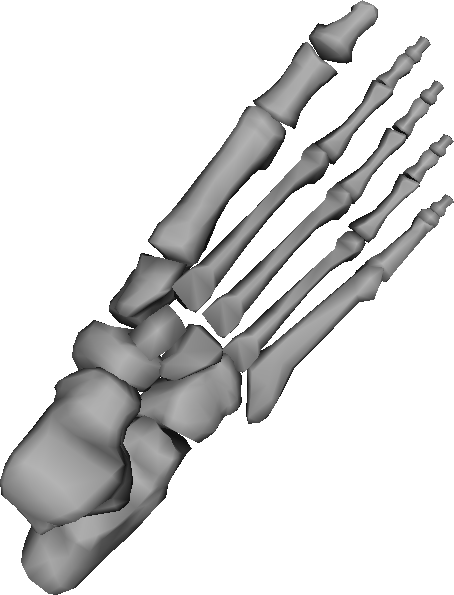
\includegraphics[width=0.45\textwidth]{pictures/image01.png}
% 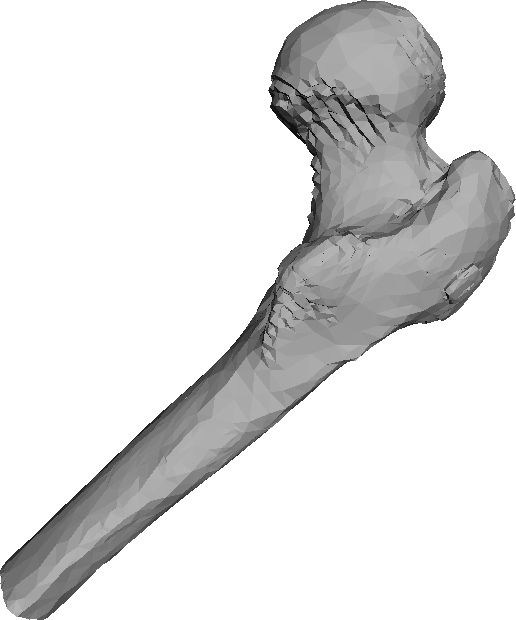
\includegraphics[width=0.45\textwidth]{pictures/image02.png}
% \caption{Meshes generated from medical data. Data obtained from the AIM$@$SHAPE Shape Repository \cite{AIMSHAPE}}
% \label{fig:example}
% \end{figure}


This document is structured as follows. In Chapter~\ref{cha:Previous Work} we present some previous work relevant to our problem. In Chapter~\ref{cha:Proposal} we explain our proposal. In Chapter~\ref{cha:Results} we show our results. Finally, in Chapter~\ref{cha:Conclusion} we present our conclusion and future work.


